\documentclass[a4paper, 10pt]{article}

\usepackage[T1]{fontenc}
\usepackage[utf8]{inputenc}
\usepackage[french]{babel}

\usepackage[top=20mm, bottom=20mm, left=10mm, right=10mm]{geometry}

\usepackage{hyperref}

\usepackage{mathpazo}
\usepackage{xcolor}
\definecolor{raspberry}{rgb}{0.737,0.067,0.259}

\usepackage{fancyhdr}
\pagestyle{fancy}

\usepackage{listings}
\usepackage{tcolorbox}
\tcbuselibrary{listings}

\newtcblisting{commandshell}{
	colback=black,
	colupper=white,
	colframe=orange!75!white,
	listing only,
	listing options={style=tcblatex,language=sh},
	every listing line={
		\textcolor{green}{\small\ttfamily\bfseries pi@raspberrypi}:\textcolor{blue}{\small\ttfamily\bfseries \~\ \$\ }
	}
}

\fancyhead[L]{\today}
\fancyhead[C]{\textit{Premiers pas avec Raspberry Pi}}
\fancyhead[R]{Swarm Drone Flight}
\fancyfoot[L]{Florian Pouthier}
\fancyfoot[R]{\jobname.pdf}
\headheight = 15pt

\begin{document}

\begin{center}
\LARGE{\textbf{Premiers pas avec Raspberry Pi}}
\end{center}

Le projet \textit{Swarm Drone Flight} nécessite l'utilisation d'un
\textbf{Raspberry Pi} embarqué sur le drone \textit{master} de l'essaim.
Ce tutoriel est là pour lister les premières étapes de prise en main
du micro-ordinateur qui agit comme le \textit{"cerveau"} de l'essaim
de drones. 

\section{Faire une image de l'OS de la RPi}

La première étape est de faire une image d'OS du RPi sur une
carte SD. Le logiciel utilisé ici est \textbf{Raspberry Pi Imager}.

\begin{enumerate}
	\item\textbf{Insérer la carte SD dans le PC.} La carte SD insérée peut
	être vierge ou non, dans tous les cas le support sera formaté au cours
	du processus. 
	
	\item\textbf{Lancer Pi Imager.} La fenêtre principale du logiciel 
	devrait ressembler à la capture de la \textsc{Figure \ref{sc_pi_imager}}.
	
	\begin{figure}[h]
		\centering
		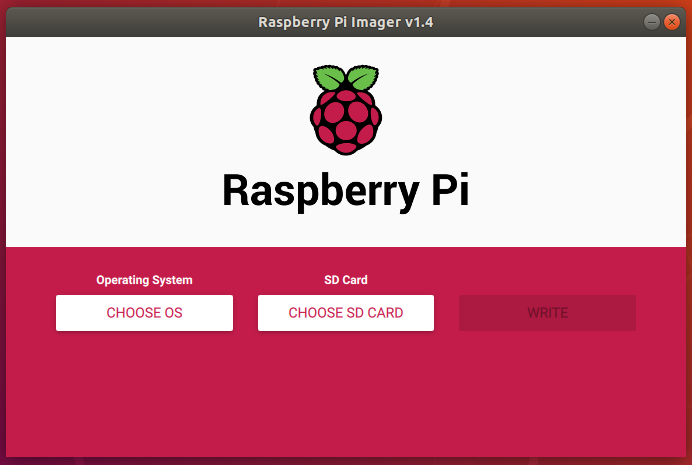
\includegraphics[scale=0.4]{fig/sc_pi_imager.png}
		\caption{Fenêtre principale de Raspberry Pi Imager.}
		\label{sc_pi_imager}
	\end{figure}

	\item\textbf{Choisir l'OS du RPi.} Nous allons installer un OS Lite,
	qui sera largement suffisant pour ce projet. Cliquer sur \texttt{CHOOSE OS}, 
	puis aller dans la liste \texttt{Raspberry Pi OS (other)}. 
	Dans cette liste, sélectionner \texttt{Raspberry Pi OS Lite (32-bit)}.
	
	\item\textbf{Choisir la carte SD.} Cliquer sur \texttt{CHOOSE SD CARD}, puis
	sur le périphérique SD qui devrait apparaître dans la liste.
	
	\item\textbf{Écrire la carte SD.} Cette fois-ci la fenêtre principale de 
	Pi Imager devrait ressembler à la capture de la \textsc{Figure \ref{write_pi_imager}}.
	
	\begin{figure}[h]
		\centering
		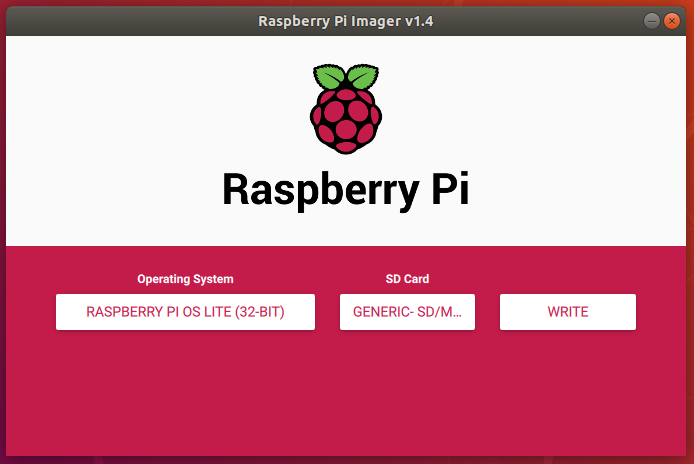
\includegraphics[scale=0.4]{fig/write_pi_imager.png}
		\caption{Fenêtre de Raspberry Pi Imager après configuration.}
		\label{write_pi_imager}
	\end{figure}
	
	Le bouton \texttt{WRITE} devient à ce moment là cliquable. Cliquer sur 
	\texttt{WRITE}, puis cliquer sur \texttt{YES} pour valider le formatage
	de la carte SD. L'écriture de la carte SD se lance alors. 
	Une fois l'écriture terminée, cliquer sur \texttt{CONTINUE}. 
	Vous pouvez maintenant retirer la carte SD de votre PC et l'insérer
	dans votre Raspberry Pi.
\end{enumerate}

\vspace{-3em}

\section{Premier démarrage du RPi}

\vspace{-0.5em}

Il est maintenant temps de travailler avec votre Raspberry Pi !

\begin{enumerate}
	\item\textbf{Brancher tous les périphériques nécessaires.} Brancher dans
	un premier temps tous les périphériques qui seront utiles pour le
	premier démarrage de votre RPi :
	
	\begin{itemize}
		\vspace{0.5em}
		\item[$\bullet$] \textbf{Ports USB :} un clavier, si besoin une souris
		mais ce n'est pas vraiment nécessaire pour un OS Lite.
		\vspace{0.5em}
		\item[$\bullet$] \textbf{HDMI :} un écran, un adaptateur VGA/HDMI peut
		s'avérer nécessaire si l'écran ne dispose que d'une connectique VGA.
		\vspace{0.5em}
		\item[$\bullet$] \textbf{Ethernet :} Si vous ne souhaitez pas utiliser
		le Wi-Fi vous pouvez vous connecter à Internet via un câble ethernet.
		Dans tous les cas, une connexion internet sera requise pour suivre ce
		tuto en intégralité.
		\vspace{0.5em}
	\end{itemize}
	
	\item\textbf{Insérer la carte SD sur le RPI.} A faire avant de mettre le
	micro-ordinateur sous tension !
	
	\item\textbf{Mettre le RPI sous tension.} Le RPi est à alimenter via le
	connecteur micro-USB. Il faut avoir un adaptateur secteur pouvant délivrer
	au minimum 2.5A, au risque de sous-alimenter le micro-ordinateur.
\end{enumerate}

D'autres informations utiles sur la prise en main du Raspberry Pi sont 
disponibles à cette adresse :
\url{https://projects.raspberrypi.org/en/projects/raspberry-pi-getting-started/}

\vspace{-1em}

\section{Première connexion au RPi}

\vspace{-0.5em}

\textit{Si vous êtes déjà familier avec les environnements Linux, vous 
verrez que la plupart des commandes sont semblables à celles utilisées 
dans un terminal Linux.}

\begin{enumerate}
	\item\textbf{Premier login.} Une fois le micro-ordinateur sous tension, 
	vous verrez à l'écran le démarrage de tous les services du RPi. 
	Une fois tous les services chargés, vous serez invités à renseigner un 
	login et un mot de passe.
	
	\textbf{raspberrypi login:} \texttt{pi}

	\textbf{Password:} \texttt{raspberry}

	Le clavier étant par défaut paramétré en QWERTY, la tentative de connexion 
	devrait échouer. En effet, il faudra saisir \texttt{rqspberry} pour pouvoir 
	réussir à se logger.
	
	\item\textbf{Changer le clavier en AZERTY.} On va tout de suite régler 
	ce problème de clavier pour terminer serainement le tuto. 
	Taper la commande suivante pour accéder au menu de configuration du RPi :
	
\begin{commandshell}
sudo raspi-config
\end{commandshell}
	
	\textit{(Saisir en réalité}\
	\texttt{sudo rqspi-config}\
	\textit{pour que ça fonctionne).}
	
	Dans le menu de configuration, sélectionner successivement :

	\begin{itemize}
		\item[$\bullet$] \texttt{4 Localisation Options} 
						 $\rightarrow$ \textbf{ENTER}
		\item[$\bullet$] \texttt{I3 Change Keyboard Layout}
						 $\rightarrow$ \textbf{ENTER}
		\item[$\bullet$] \texttt{Generic 105-Key PC (int1.)}
						 $\rightarrow$ \textbf{ENTER}
		\item[$\bullet$] \texttt{Other}
						 $\rightarrow$ \textbf{ENTER}
		\item[$\bullet$] \texttt{French}
						 $\rightarrow$ \textbf{ENTER}	
		\item[$\bullet$] \texttt{French}
						 $\rightarrow$ \textbf{ENTER}	
		\item[$\bullet$] \texttt{The default for the keyboard layout}
						 $\rightarrow$ \textbf{ENTER}	
		\item[$\bullet$] \texttt{No compose key}
						 $\rightarrow$ \textbf{ENTER}			 		
	\end{itemize}
	
	Vous revenez finalement au menu principal de configuration.
	
	\item\textbf{Configurer le Wi-Fi.} Si vous n'avez pas de connexion
	ethernet, vous devez configurer une connexion au réseau Wi-Fi pour
	pouvoir accéder à internet. Pour cela, toujours dans le menu de
	configuration, sélectionner successivement :

	\begin{itemize}
		\item[$\bullet$] \texttt{2 Network Options} 
						 $\rightarrow$ \textbf{ENTER}
		\item[$\bullet$] \texttt{N2 Wireless LAN}
						 $\rightarrow$ \textbf{ENTER}
		\item[$\bullet$] \texttt{FR France}
						 $\rightarrow$ \textbf{ENTER}
		\item[$\bullet$] \texttt{<OK>}
						 $\rightarrow$ \textbf{ENTER}
		\item[$\bullet$] \texttt{Please enter SSID}
						 $\rightarrow$ Saisir le nom du réseau Wi-Fi
						 $\rightarrow$ \textbf{ENTER}	
		\item[$\bullet$] \texttt{Please enter passphrase}
						 $\rightarrow$ Saisir le mot de passe du Wi-Fi
						 $\rightarrow$ \textbf{ENTER}		 		
	\end{itemize}
	
	Vous revenez finalement au menu principal de configuration.
	Pour sortir du menu, sélectionner \texttt{<Finish>}
	$\rightarrow$ \textbf{ENTER}.	

	\item\textbf{Redémarrer le RPi.} Pour prendre en compte les 
	différentes modifications précédentes, redémarrer le RPi avec
	la commande suivante :	
	
\begin{commandshell}
sudo reboot
\end{commandshell}	

	Ressaisir finalement le login \texttt{pi} et le mot de passe \texttt{raspberry}. 
\end{enumerate}

\section{Installation des packages}

Pour travailler sur le projet \textit{Swarm Drone Flight}, il faut
installer certains packages qui ne sont pas initialement installés
dans l'OS Lite.

\begin{enumerate}
	\item\textbf{Vérifier la connexion internet.} La connexion internet 
	peut être rapidement vérifiée en faisant un \texttt{ping} sur un
	site web quelconque.
	
\begin{commandshell}
ping google.fr
\end{commandshell}

	Si des lignes de réception de paquets apparaissent, alors la
	connexion internet est bien établie ! Sinon vérifier que les
	login et mot de passe du réseau Wi-Fi ciblé sont bien paramétrés
	en refaisant la procédure décrite à la page précédente.	
	Arrêter le processus avec \textbf{Ctrl} + \textbf{C}.
	
	\item\textbf{Mettre à jour l'OS.} Afin d'obtenir la dernière version
	de l'OS, saisir :
	
\begin{commandshell}
sudo apt-get upgrade
\end{commandshell}
	
	Un message demandant si vous autorisez le téléchargement de paquets
	devrait également apparaître, valider en appuyant \textbf{ENTER}.
	
	\item\textbf{Installer GitHub}. Installer \texttt{GitHub} pour le 
	versionning des codes utilisés en saisissant :
	
\begin{commandshell}
sudo apt-get install git
\end{commandshell}	
	
	\item\textbf{Installer Python 3}. Afin d'installer \texttt{Python 3},
	saisir :
	
\begin{commandshell}
sudo apt-get install python3
\end{commandshell}

	\item\textbf{Charger l'installateur de paquets Python 3}. 
	L'installateur de paquets \texttt{Python 3} peut être chargé avec :
	
\begin{commandshell}
sudo apt-get install python3-pip
\end{commandshell}

	\item\textbf{Installer le paquet \texttt{dronekit}}. 
	Le paquet \texttt{dronekit} permet la communication avec un
	contrôleur de vol (un \textit{Pixhawk} par exemple) en 
	utilisant un protocole MAVLink.
	
\begin{commandshell}
pip3 install dronekit
\end{commandshell}
\end{enumerate}

\end{document}